% \documentclass[10pt, english, pdftex]{template/UC3M_document}
\documentclass[10pt, spanish, pdftex]{template/UC3M_document}

%%%%% Preamble %%%%%
\author{Alejandro Prieto Macías}         % This is me! You should write here your name (for PDF metadata)
%%%%% About the authors (will be used on title page and header) %%%%%

%%% Indicate the number of authors by uncommenting the right option.
 \authorstwotrue     % 1 or 2 authors
% \authorsthreetrue   % 3 authors
%\authorsfourtrue    % 4 authors

%%% Fill with the authors data. You can leave empty keys {} if you need to and also if you provide more info that number of authors indicated it will be ignored.
% If you selected \authorstwotrue or \authorsthreetrue (1 to 3 authors)
\authorsuptothree{Alejandro Prieto Macías}{NIA 100383428}{Gr. 81}{Alejandro Valverde Mahou}{NIA 100383383}{Gr. 81}{Name3 Lastname3}{NIA 100XXXXXX}{Gr. XX}
% If you selected \coauthorsfourtrue (4 authors)
\authorsfour{Name1 Lastname1}{NIA 100XXXXXX}{Name2 Lastname2}{NIA 100XXXXXX}{Name3 Lastname3}{NIA 100XXXXXX}{Name4 Lastname4}{NIA 100XXXXXX}{Group XX}

%%% If you want to show coauthors email address on the title page, uncomment \emailtrue. Comment it otherwise.
%\emailtrue
% You can leave empty keys {} if you need to and also if you provide more info that number of authors indicated or \emailtrue is commented it will be ignored.
\emails{email1@domain.tld}{email2@domain.tld}{email3@domain.tld}{email4@domain.tld}


%%%%%%%%PARA EL mybox%%%%%%%%%%%%%%%%%%%%%%%%%%%%%%%%%%%%%%%%%%%%%%%%
% Cuadros de colores
\usepackage{tcolorbox}
\usepackage{wrapfig}
\usepackage{hyperref}

\newtcolorbox{boxAntonio}[2]
{colback=#2!5!white,colframe=uc3mDarkBlue,fonttitle=\bfseries,title=#1, flushleft title, width=\linewidth, height=5.7cm}
\newtcolorbox{boxSara}[2]
{colback=#2!5!white,colframe=uc3mDarkBlue,fonttitle=\bfseries,title=#1, flushleft title, width=\linewidth, height=4.8cm}
\newtcolorbox{boxCarla}[2]
{colback=#2!5!white,colframe=uc3mDarkBlue,fonttitle=\bfseries,title=#1, flushleft title, width=\linewidth, height=6.15cm}
%%%%%%%%PARA EL mybox%%%%%%%%%%%%%%%%%%%%%%%%%%%%%%%%%%%%%%%%%%%%%%%%


%%%%% Basic data about the document (Degree, subject, title, campus, page number custom text) %%%%%
\documentdata{Ingeniería Informática}{Interfaces de Usuario}{Práctica Final}{Leganés}{}

%%%%% Page style %%%%%
\header
\footer
\pagestyle{fancy}


\begin{document}
%%%%% Page title %%%%%
\titleMain

%%%%% Index %%%%%
\begin{spacing}{0.5}
    % \shipout\null                   % Blank page before index (after title page)
    \hypersetup{linkcolor=black}    % References/links on the index will remain black color
    \tableofcontents\newpage        % Index of the document
    % \listoffigures\newpage          % Index of pictures
    % \listoftables\newpage           % Index of tables
\end{spacing}


%%%%% DOCUMENT CONTENT %%%%%
\section{Objetivo}
El objectivo de este ejercicio es diseñar una plataforma para seguir e informarse sobre las actividades del \href{http://www.cplmadrid.com}{club de hockey CPL Madrid}.

\newpage

\section{Usuarios y Entorno}
\subsection{Conoce al Usuario}
Es importante definir a los posibles usuarios de la plataforma. Para ello vamos a modelizar a tres de ellos: un padre, un jugador y un posible inversor interesado en el equipo.

\subsubsection{José Antonio}
\begin{boxAntonio}{}{blue}
  \begin{wrapfigure}{l}{0.2\textwidth}
  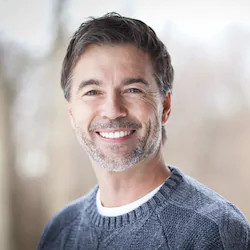
\includegraphics[scale=1.5]{Images/Antonio.jpg}
  \caption{José Antonio}
  \end{wrapfigure}
  \small José Antonio es un hombre de 45 años que tiene dos hijos que juega en el club CPL Madrid. En un entusiasta del hockey y le gusta seguir las ligas tanto de su hijo, como la de su hija. Este año le ha tocado ser el delegado del equipo de su hija, el equipo Benjamín. Por lo tanto, le toca subir las crónicas de los partidos en la página web del equipo. No se maneja demasiado bien con las tecnologías y por eso necesita que la web sea sencilla y fácil de usar. El móvil no es una herramienta para él, por eso prefiere revisar los partidos desde el PC del trabajo. También, necesita saber donde está la información que incumbe a los partidos de sus hijos, para saber cuándo y a dónde les tiene que llevar a jugar. \break
  Como siempre dice José Antonio:
  \textbf{"Con trabajo, trabajo, trabajo y mucho esfuerzo, se consiguen los sueños."}
\end{boxAntonio} \hfill \break

\subsubsection{Sara}
\begin{boxSara}{}{blue}
 \begin{wrapfigure}{l}{0.2\textwidth}
 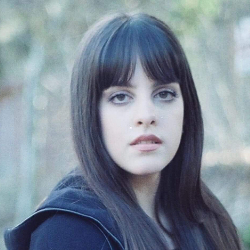
\includegraphics[scale=1.5]{Images/Sara.jpg}
 \caption{Sara}
 \end{wrapfigure}
 \small Sara es una joven de 17 años que juega en el club CPL Madrid en la sección femenina, Walkyrias. Es una chica un poco pasota, no tiene mucho interés en el resto de sus compañeras. Pero le encanta ver las estadísticas de sus temporadas anteriores, pues ya lleva 8 en el club, y ver que siempre ha estado la primera. Se pasa el día pegada al smartphone, cuando tiene partido lo consulta desde ahí para decírselo a sus padres. Puesto que le tienen que llevar al campo en coche.
 No tiene lema personal, pero siempre dice que \textbf{es la mejor}.
\end{boxSara}

\subsubsection{Carla}
\begin{boxCarla}{}{blue}
  \begin{wrapfigure}{l}{0.2\textwidth}
  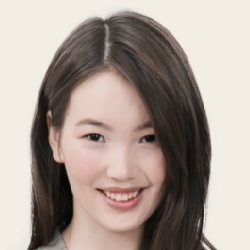
\includegraphics[scale=1.5]{Images/Carla.jpg}
  \caption{Carla}
  \end{wrapfigure}
  \small Carla es una joven emprendedora que trabaja para una compañía grande de móviles, y le han encargado que consiga que algún club deportivo de la Comunidad de Madrid lleve el logo de la empresa en la camiseta a modo de promoción. Carla ha encontrado de casualidad el sitio web del CPL Madrid. Ella busca un club ganador para poder llegar a la máxima cantidad de personas y con suerte aparecer en un periódico nacional. En el sitio web lo que quiere saber es la clasificación que ha conseguido el equipo en los últimos años. También necesita saber como ponerse en contacto con el club, además de su historia y que es lo que hacen. Carla trabaja a través de múltiples dipositivos: su smartphone, su tablet y su portátil. Lleva toda su vida usando las tecnologías, y está muy familiarizada con ellas.
  Carla solo tiene una cosa en mente, conseguir el puesto de CEO de la empresa trabajando desde abajo. En sus redes sociales siempre tiene de estado \textbf{"Go big or go home"}.
\end{boxCarla}

%Fin de sección de Usuarios
\pagebreak

\subsection{Entorno}
Para este apartado se han buscado sitios web de clubes grandes de los que conocemos que su diseño nos parece correcto para proceder con su análisis. Esto será de gran utiliadad para el desarrollo de nuestra propia aplicación, en este caso del sitio web que debemos renovar.
\subsubsection{Sitio web actual de \href{http://www.cplmadrid.com/}{CPL Madrid}}
En primer lugar, hemos analizado las funcionalidades de la propia web que debemos renovar.
\paragraph{Heurística de Nielsen}
\begin{itemize}
  \item \textbf{Visibilidad del estado del sistema}

  El sistema informa, a través de la barra de navegación, de la posición del usuario. Además, al visitar una subsección aparece un \textit{rastro de miga de pan}.

  \item \textbf{Coincidencia entre el sistema y el mundo real}

  El sistema no posee herramientas en las que exista coincidencia con el mundo real.

  \item \textbf{Control y libertad de los usuarios}

  El sistema no proporciona herramientas para regresar al estado anterior en caso de error o equivocación, más allá de la barra de navegación en algunos casos.

  \item \textbf{Consistencia y estándares}

  El sitio web no sigue las reglas de consistencia llegando a utilizar diferentes estilos e incluso duplicando las herramientas navegación.

  \item \textbf{Prevención de errores}

  No posee un sistema de prevención de errores. Tampoco es necesario puesto que la interacción del usuario simplemente es navegar por las distintas páginas.

  \item \textbf{Minimizar la carga de la memoria del usuario}

  El sistema no obliga al usuario a recordar cómo usar el sitio. La navegación resulta intuitiva.

  \item \textbf{Flexibilidad y eficiencia de uso}

  La diferencia entre un usuario nuevo y uno experimentado no es grande, pero el experimentado podría encontrar apartados con mayor agilidad.

  \item \textbf{Diálogos estéticos y diseño minimalista}

  El diseño es antiguo, poco cuidado e inconsistente.

  \item \textbf{Ayudar a los usuarios a reconocer, diagnosticar y recuperarse de los errores}

  No posee tampoco un sistema de recuperación de errores, pueden resultar inesperados y la solución es ir atrás con los botones propios del navegador.

  \item \textbf{Ayuda y documentación}

  Tampoco cuenta con ayuda ni documentación extra.
\end{itemize}
\paragraph{Patrones de Diseño de Van Duyne}
  \begin{itemize}
    \item \textbf{A12: Blogs}

    El sitio web tiene una estructura de blog porque tiene diferentes entradas organizadas en una lista.
    La aplicación cumple con el patrón de diseño de mantener la página como algo personal, y que permite los comentarios de los usuarios.
    Por el contrario, no cumple el hacer sencillo encontrar la información, ya que está muy desorganizado, y no posee ningún filtro.

    \item \textbf{B8: Páginas organizadas por categoría}

    El sitio web está organizado por categorías, porque cada pestaña de la aplicación constituye un apartado diferente completamente del resto.
    Aunque está organizado de esta forma, no cumple los patrones de diseño necesarios, ya que no usa un \textit{layout} consitente, ya que el formato cambia entre pestañas. Tampoco mantiene el método de navegación, ya que, dependiendo en el apartado en el que se encuentre el usuario, la barra de navegación cambia de diseño y de posición. Solo informa de la posición del usuario en algunas de las categorías, usando títulos resaltados.

    \item \textbf{E5: Sobre nosotros}

    El sitio web posee de un apartado de \textit[Conócenos], donde aparece toda la información relevante del club de hockey.

    \item \textbf{I6: Consistencia en el contenido de los \textit{sidebar}}

    En casi todas las pesañas de la apliación aparecen unas \textit{sidebar} con contenido que puede ser interesante para los usuarios en todo momento. Esto facilita el acceso de los usuarios. Su posicionamiento se mantiene siempre a la derecha de la página, y tienen siempre la misma longitud, que es menor al tamaño máximo del sitio web.

    \item \textbf{J1: Búsqueda de acciones dentro de la página}

    El sitio web cuenta con un buscador con herramientas de búsqueda de \textit{Google}. Está colocado en una posición visible: En la parte superior de la página.

    \item \textbf{K2: Barra de navegación}

  \end{itemize}

\subsubsection{Sitio web del \href{https://www.atleticodemadrid.com/}{Atlético de Madrid}}
En segundo lugar, nos ha parecido oportuno optar por revisar la web de este club puesto que sabemos que tiene caracterísitcas que podían ser útiles.

\paragraph{Heurística de Nielsen}
\begin{itemize}
  \item \textbf{Visibilidad del estado del sistema}

  El sitio muestra el título de la sección visitada. Además, de un \textit{rastro de miga de pan}, pero no resulta claro.

  \item \textbf{Coincidencia entre el sistema y el mundo real}

  El sistema no posee herramientas en las que exista coincidencia con el mundo real.

  \item \textbf{Control y libertad de los usuarios}

  El sistema proporciona libertad y control satisfactorio de la web. A excepción, de algunos casos que debido al formato de la pantalla no se pueden visitar.

  \item \textbf{Consistencia y estándares}

  El sitio web mantiene un estilo constante y no varía en función de la acción que el usuario esté haciendo.

  \item \textbf{Prevención de errores}

  En el caso de que el usuario quiera comprar una entrada y se equivoque de partido, no hay manera de retornar a la lista de partidos teniendo que cerrar la pestaña del navegador.

  \item \textbf{Minimizar la carga de la memoria del usuario}

  El sistema no obliga al usuario a recordar cómo usar el sitio. La navegación resulta intuitiva.

  \item \textbf{Flexibilidad y eficiencia de uso}

  La diferencia entre un usuario nuevo y uno experimentado es grande puesto que el contenido de la web es amplio y un usuario experimentado se maneja mucho mejor.

  \item \textbf{Diálogos estéticos y diseño minimalista}

  El diseño es muy bueno, consistente, aunque en algunos casos demasiado recargado.

  \item \textbf{Ayudar a los usuarios a reconocer, diagnosticar y recuperarse de los errores}

  En caso de error resulta fácil e intuitivo regrasar al estado anterior.

  \item \textbf{Ayuda y documentación}

  No cuenta con ayuda al usuario, pero posee documentación tales como \textit{política de privacidad y de cookies}.
\end{itemize}

\paragraph{Patrones de Diseño de Van Duyne}
\begin{itemize}
  \item \textbf{A7: Compañías de valores}

  El sitio web es el de un equipo deportivo de gran relevancia nacional e internacional, y tiene una organización adecuada para sus fans. Estos son también clientes puesto que compran merchandising y entradas, por ello encontramos un apartado para la tienda y uno específico para las entradas permitiendo un acceso intuitivo.

  \item \textbf{B2: Contenido navegable}

  El sistema posee un menú por el que navegar y poder cambiar entre diferentes categorías fácilmente.

  \item \textbf{B6: Organización cronológica}

  El sistema posee una organización cronológica necesaria en el calendario de partidos, resulta intuitiva puesto que te dirige al último partido cuando visitas el calendario y en caso de necesitar una fecha anterior con hacer scroll hacia arriba bastaría. Al igual ocurre si necesitas una fecha posterior. Además, las noticias están organizadas de tal manera que las más recientes aparecen en primer lugar.

  \item \textbf{B7: Organización basada en la popularidad}

  El menú tiene varias opciones organizadas en orden de interés, en primer lugar encontramos la información del equipo masculino, puesto que posee más historia y más seguidores. En segundo lugar, el equipo femenino, que tiene una menor relevancia menor en cuanto a número de fans, pero es importante. En tercer lugar, aparece el apartado \textit{Academia} en el que se consultan los resultados de los filiales. Y después encontramos el resto de opciones que resultan menos relevantes, pero que necesitan ser accecibles.

  \item \textbf{C1: Construcción de una marca}

  Uno de los objetivos de la web es vender la marca del equipo y para ello poseen anuncios de sus propios productos.

  \item \textbf{D1: Plantilla de página}

  La aplicación ha aplicado la misma plantilla para todas las páginas. El diseño es continuo, mantiene los colores, logos en todo momento con un mismo estilo. Los estilos de los menús son similares en todo momento mantiendo una clara coherencia.

  \item \textbf{D10: Internacionalización}

  El sito web varía su contenido según el idioma que se indique. Por ejemplo, en chino el contenido es muy distinto cambiando la barra de navegación incluso. Aunque mantiene la plantilla de aspecto.

  \item \textbf{J3: Búsqueda organizada}

  El sitio posee una herramienta de búsqueda, pero resulta bastante inútil. Los resultados mostrados no parecen seguir un patrón más allá de la temporalidad.
  \item \textbf{M1: Mobile screen}

  El diseño está muy cuidado y pensado para ser responsive. El contenido esa accesible y perfectamente legible y adaptable.

\end{itemize}
%Fin de sección de Entorno
\newpage

\section{Prototipo e Implementación}
Durante la realización del proyecto, hemos intento atenernos al máximo al diseño realizado en el prototipo.
En algunos casos se ha seguido feacientemente, pero en otros se ha modificado para adaptarlo a un diseño que correspondiese con alguna heurística o patrón con el fin de mejorar el sitio. En otros casos, por estética o funcionalidad hemos decido adoptar otro estilo. En cualquier caso, el estilo básico y estructural se ha mantenido en todo momento.

Las heurísticas y patrones descritos son los que se han incluido en el diseño de la implementación. Por tanto.
\subsection{Primer prototipo}
En nuestro caso, al desarrollar un proyecto diferente al resto de compañeros, no hemos conseguido juntarnos con otro grupo y por tanto, decidimos que nuestro prototipo (\textit{el de la práctica 3}) era el adecuado como base para la \textit{Práctica Final}.

\subsection{Presentación del prototipo Final}
  \subsubsection{Página principal}
  \begin{figure}[H]
    \centering
    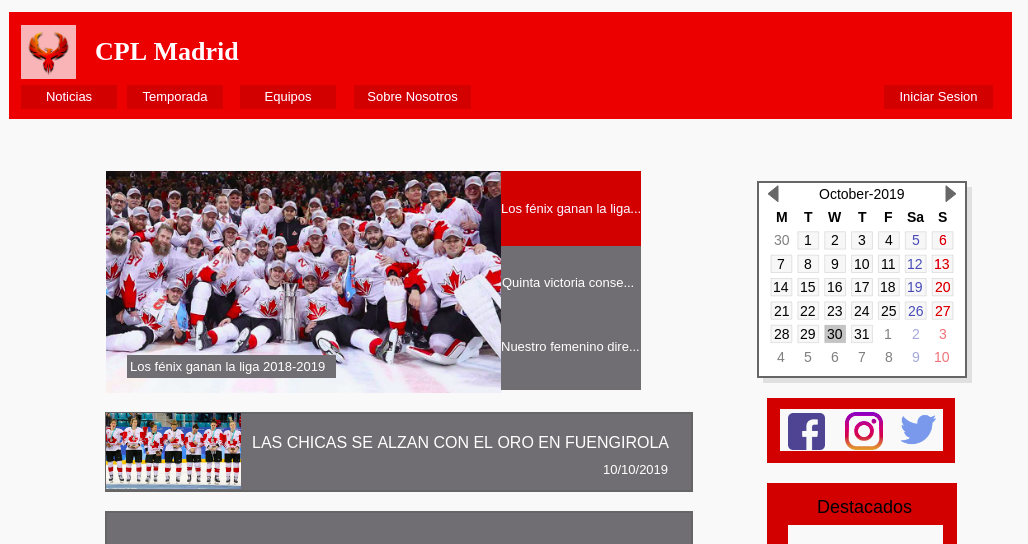
\includegraphics [width=18.5cm] {Images/Prototipo/home.png}
    \caption{Home}
  \end{figure}

  \subsubsection{Noticias y creación de entradas}
  \begin{figure}[H]
    \centering
    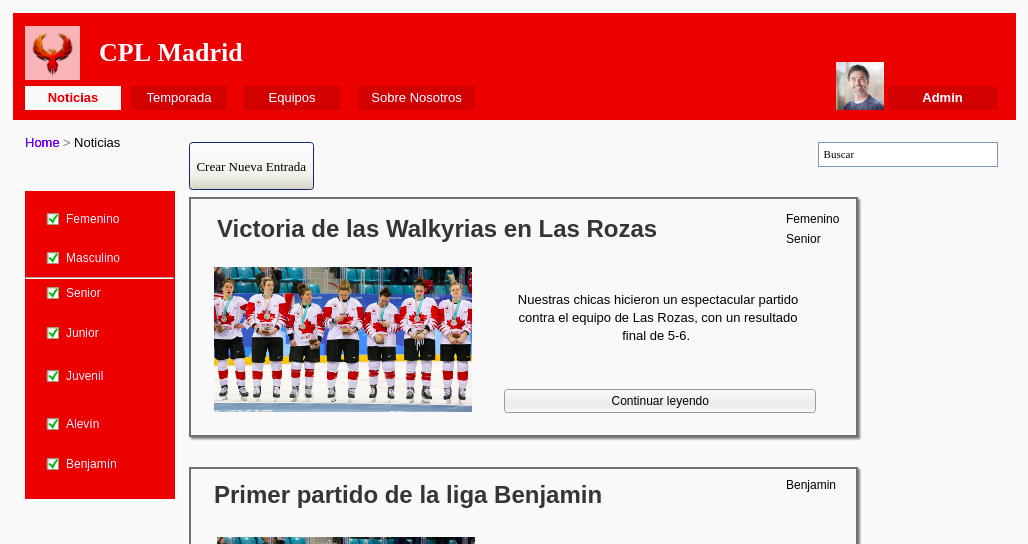
\includegraphics [width=18.5cm]{Images/Prototipo/noticias.png}
    \caption{Noticias}
  \end{figure}

  \begin{figure}[H]
    \centering
    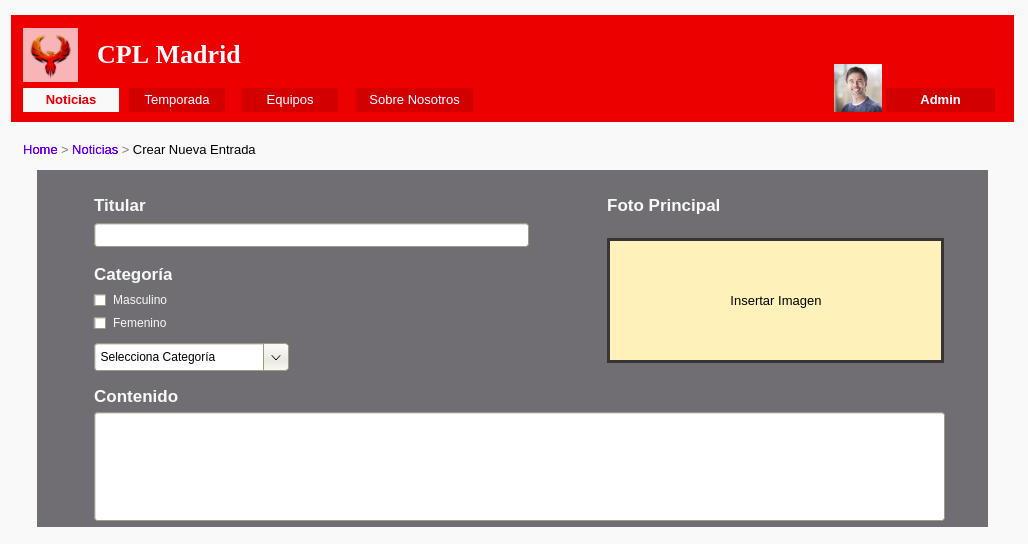
\includegraphics [width=18.5cm] {Images/Prototipo/crear_entrada.png}
    \caption{Nueva noticia}
  \end{figure}

  \subsubsection{Clasificaciones Versión Móvil y Desktop}
  \begin{figure}[H]
    \centering
    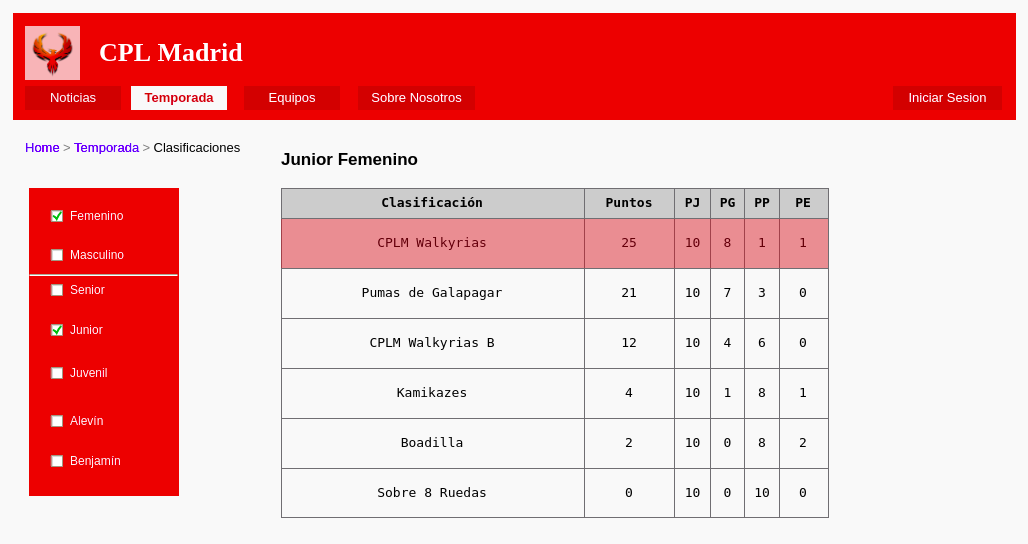
\includegraphics [width=18.5cm] {Images/Prototipo/clasificaciones.png}
    \caption{Clasificaciones Desktop}
  \end{figure}

  \begin{figure}[H]
    \centering
    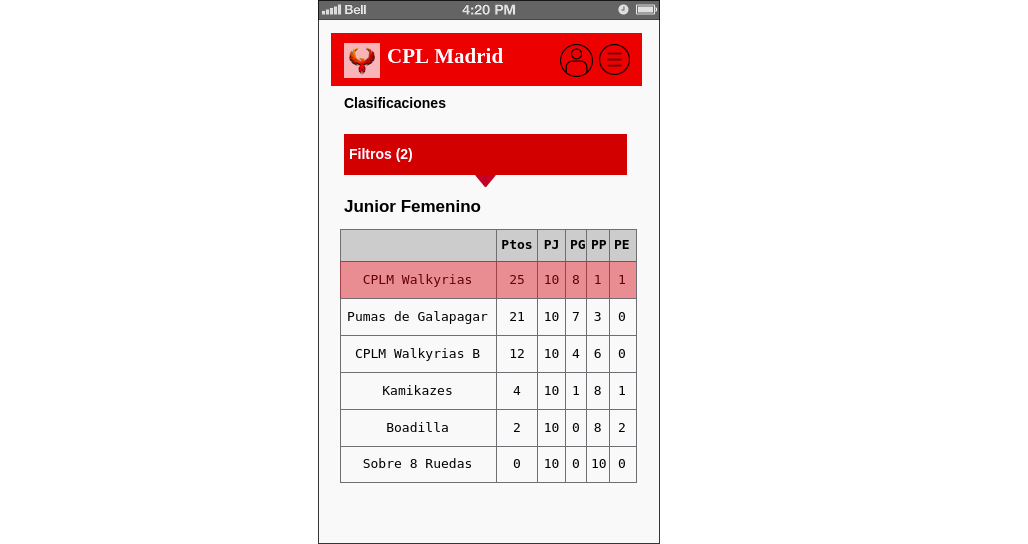
\includegraphics [width=18.5cm] {Images/Prototipo/clasificaciones_mvil.png}
    \caption{Clasificaciones Móvil}
  \end{figure}



\subsection{Implementación}
Vamos a desarrollar brevemente el reparto de tareas y el flujo de trabajo que se ha llevado a cabo.

\textbf{NOTA:} Para iniciar sesión, usar \textbf{Usuario} \textit{FanFenix} y \textbf{Contraseña} \textit{admin}.

\subsubsection{Colores}\label{paleta}
Uno de los primeros pasos fue la elección de colores que siguieran la estética del club al que representa el sitio web, pero siguiendo los principios de usar tres colores básicos y dos extra que deriven de ellos. Para ello, hemos usado software externo para la creación de la paleta.

\subsubsection{Estructura}
Tras realizar una encuesta y hablar con el cliente, \textbf{el club CPL Madrid}, tuvo que rediseñarse la barra de navegación y añadir un apartado extra que el cliente consideraba imprescindible. Además, la encuesta nos permitió enfocar el desarrollo hacia las zonas que necesitaban ser más púlidas y que tenían que tener funcionalidad.

Por otro lado, en el apartado de noticias los filtros de noticias fueron eliminado a petición del cliente. Además, se nos puso como requisito crear un superusuario que pudiera manejar al resto de usuarios y administralos. Esta funcionalidad no ha sido completada, puesto que tiene que ser desarrollado con servidores a los cuales todavía no nos han permitido el acceso y por tanto el desarrollo del \textit{back-end} no ha sido posible.

A continuación, se explicarán las secciones que presenta el sitio web y las que han sido desarrolladas se explicarán en mayor profundidad.

\paragraph{Index}
Se trata de la página principal del sitio, en ella se muestran las últimas noticias subidas al sitio. En el carousel se indican las tres últimas y posteriormente aparecen las dos siguientes.
En el lateral se muestran elementos de utilidad para el usuario, un apartado de destacados(modificable por los administradores), enlaces a las federaciones de Hockey Linea, el calendario de eventos y redes sociales.
\paragraph{Noticias}
Aquí se añaden las noticias creadas, en esta sección se muestra un resumen de las noticias y el enlace para leerla por completo.

Los administradores podrán ver un botón para crear una nueva noticia, que lleva a otra página especial para crear noticias. Actualmente, se crea una previsualización de la noticia, pero no permite publicarla. Además, si mientras se crea la noticia se cierra la sesión, redirige a la página principal puesto que solo si eres administrador tienes permiso para crear entradas nuevas.
Los administradores también pueden eliminar noticias mediante el botón de eliminar que se muestra al Iniciar Sesión.
\paragraph{Temporada}
Este apartado no tiene desarrollado el contenido actualmente

\paragraph{Equipo}
Este apartado no tiene desarrollado el contenido actualmente

\paragraph{Patinaje}
En este apartado, se muestra información acerca de los cursos que se imparten en el recinto de patinaje. Los administradores tienen permiso para eliminar contenido mediante el botón habilitado.

\paragraph{Sobre Nosotros}
En esta sección se muestran tenemos un formulario de contacto en caso de querer comunicarse con el club. Actualmente, no envía correo porque no tiene una base de datos para poder realizar estas peticiones.

Y por otro lado, información de la historia del equipo, además de incluir imágenes.
Los usuarios registrados pueden eliminar tarjetas de información.

\paragraph{Usuario}
Este apartado, muestra un formulario dividos en varias partes. En estas se permite cambiar el nombre de usuario y la contraseña del administrador actual. Además, esta cuenta puede eliminarse.

Desde el usuario, se pueden crear más administradores de la web para distribuirlos a más personas.

Actualmente, para esta entrega, no es funcional ya que requiere de una base de datos para manejar los usuarios nuevos, así como los cambios.




\subsubsection{Flujo de trabajo}
\paragraph{Proyecto}


Para realizar esta práctica se ha creado un proyecto en GitHub (\url{https://github.com/Pheithar/FanFenix}) en el que se han creado los requisitos y apartados a desarrollar.
\paragraph{Reparto de tareas}


Se han asignado tareas y mediante reuniones o trabajando juntos, se han acordado la guía a seguir para obtener coherencia.


\subsection{Heurísticas de Nielsen}
  \begin{itemize}
    \item \textbf{Visibilidad del estado del sistema}
    El sitio posee un indicador en la barra de navegación que indica en qué apartado se encuentra el usuario en todo momento. A excepción, de la pantalla principal que no posee este indicador negro.
    Además, pose un texto que indica la subseción (o sección principal en caso de no haber ninguna) en la que el usuario se encuentra.

    \item \textbf{Coincidencia entre el sistema y el mundo real}
    El sistema no posee herramientas en las que exista coincidencia con el mundo real.

    \item \textbf{Control y libertad de los usuarios}
    El usuario de tipo visitante, no tiene libertad más allá de navegar por las pestañas que desee.

    \item \textbf{Consistencia y estándares}
    El sitio web mantiene un estilo constante y no varía en función de la acción que el usuario esté haciendo.

    \item \textbf{Prevención de errores}
    El sistema provee al usuario una alerta de confirmación a la hora de eliminar una noticia y al cerrar sesión.

    \item \textbf{Minimizar la carga de la memoria del usuario}
    El sitio web tiene los apartados reconocibles para que el usuario no tenga dificultad en encontrar algo sin tener que pensar dónde suele estar.

    \item \textbf{Flexibilidad y eficiencia de uso}
    El usuario experto y el nuevo no deberían notar dificultad en la navegación. Es cierto, que si se trata de un administrador nuevo puede encontrar los botones de \textbf{Inciar Sesión} y \textbf{editar} no accecibles. Este diseño está realizado así, puesto que la mayoría de usuarios son usuarios que ven y no que editan.

    \item \textbf{Diálogos estéticos y diseño minimalista}
    Posee un diseño sencillo basado en tres colores básicos (rojo, negro y blanco-grisáceo) y con estos tres se han construido tarjetas simples para las noticias y contenido en general.

    \item \textbf{Ayudar a los usuarios a reconocer, diagnosticar y recuperarse de los errores}
    El sistema no posee apoyo en caso de error.

    \item \textbf{Ayuda y documentación}
    El sitio tiene en el footer un enlace a la documentación del proyecto en GitHub. En él se explica el desarrollo puesto que es un repositorio público y por tanto accesible para cualquiera.
  \end{itemize}


\subsection{Patrones de diseño de Van Duyne}
A continuación, se expondrán algunos de los patrones que se han tenido en cuenta durante el desarrollo del sitio web.
%%%%%%%%%%%%%%%%%%%%%%%%%%%%%%NO LO SÉ%%%%%%%%%%%%%%%%%%%%%%%%%%%%%%%%%%%%%%%%%
%\subsubsection{A: Género del sitio}
%\paragraph{A?}

\subsubsection{B: Navegación}
\paragraph{B3: Organización Jerárquica}
  El sito web posee subgrupos detrás de las ideas principales y que se indican en los desplegables de la barra de navegación. Por ejemplo, \textit{Temporada} tiene los subapartados \textit{Clasificación, calendarios, Ligas, Estadísticas} que tienen sentido lógico de ser estar recogidas en ese apartado.
\paragraph{B7: Organización basada en la popularidad}
  Los apartados principales del sitio, recogidos en la barra de navegación. Tras realizar una encuesta a los usuarios de la web actual, se ha establecido que el orden a seguir debía ser el utilizado.
\paragraph{B8: Categoría de páginas}
  Se ha aplicado un estilo general para toda la web. Cada apartado requiere una estructura distinta, pero para que crear unificación ciertas subestructuras se han adoptado con el mismo estilo o muy similar.
\subsubsection{C: Página Principal}
\paragraph{C1: Página Principal}
  El sitio web posee una página principal en la que se indica los contenidos mediante la barra de navegación en la parte superior. Justo por encima, se presenta el logo y nombre del club a los que hemos querido dar gran importancia. En la parte izquierda superior se presenta el botón de Iniciar Sesión, ya que no es una acción principal y solo lo harán unos pocos usuarios, hemos considerado que el sitio era adecuado para no quitar visibilidad al contenido.

  Además, el sitio posee una página de noticias principales, seguido de noticias secundarias hechas por módulos. En el lado, se ha colocado accesos a redes sociales, el calendario del eventos, noticias destacadas y un widget de una red social.


\subsubsection{D: Manejando contenido}
\paragraph{D1: Modelo de página}
  Todas la páginas del sitio tienen el mismo header y footer, esa es la parte principal del modelo que se aplica en todos. Posteriormente, en las páginas que poseen texto tienen unos contenedores con estilo de tarjeta unificado y apliacado como si fuera un molde.
\paragraph{D7: Estilo de pirámide invertida}
  Cada entrada del blog, está organizada con este estilo ya que se tratan de artículos de contenido de estilo periodístico que siguen estas reglas. Las noticias o entradas, tienen un titular y una foto en la parte superior que proporcionan la mayor cantidad de información. A continuación, se procede a desarrollar el contenido dejando para el final la información menos relevante.
\paragraph{D9: Título de HTML distinguibles}
  Cada subapartado tiene su propio HTML asociado con nombres únicos y explicativos.


\subsubsection{E: Construyendo confianza y credibilidad}
\paragraph{E1: Marca}
  Se ha considerado la inclusión del logo del club en todas las páginas. Además, como se comentó en el apartado de \ref{paleta} colores los colores elegidos son los del club. Estos están presentes en el escudo, tipografía y equipaciones.
\paragraph{E5: Sobre Nosotros}
  El sitio web posee un apartado llamado \textit{Sobre Nosotros} y en él se explica información del club para poner un contexto.

\subsubsection{H: Ayudando a completar tareas}
\paragraph{H2: Iniciar Sesión/ Nueva cuenta}
  La creación de cuenta solo lo podrá hacer un administrador y para crear uno nuevo simplemente se piden unas credenciales básicas en los que se deja claro que son campos de obligatoriedad.
  Por tanto, la web no necesita registro para darle un uso común, solo para los administradores que necesiten editar el contenido.
\paragraph{H3: Cuenta de Invitado}
  Como se ha explicado en el punto anterior, no es necesario tener una cuenta para visitar el sito web.
\paragraph{H10: Formularios claros}
  Los formularios no tienen una gran complejidad y posee los campos mínimos y necesarios en cada caso. El formulario para contactar con el club posee un control inteligente en caso de que algún campo obligatorio no esté completo.

\subsubsection{I: Definiendo composiciones efectivas de páginas}
\paragraph{I4: Cambiar el contenido relativo al ancho de pantalla}
  En los ordenadores, el ancho del contenido varía dependiendo del ancho de la pantalla. Por ello, es adaptable.

\subsubsection{K: Haciendo la navegación fácil}
\paragraph{K2: Barra de navegación}
  Barra de navegación presente en todas páginas para permitir la navegación entre apartados.
\paragraph{K4: Action Buttons}
  Los botones cuando se pulsan poseen una pequeña respuesta que indica que se están pulsando. Además, en formularios en los que se puede incluir alguna imagen, al lado del botón incluirá el nombre de la foto para indicar que se ha seleccionado.
\paragraph{K5: Botones de alta visibilidad}
  Los botones tienen un color rojo que permite al usuario darse cuenta más fácilmente de su existencia y facilitando la navegación.
\paragraph{K8: Link externo}
  El sitio web posee vario enlaces externos. Los más relevantes se pueden encontrar en la página principal en la que se encuentran las redes sociales del club accesibles a través de esta utilidad.
\paragraph{K9: Descriptivo}
  El sitio posee botones de \textbf{Leer más} que referencia a la noticia completa que contiene el resto de la información no accesible desde la página desde la que se navegó.
\paragraph{K11: Lenguaje familiar}
  El lenguaje utilizado está relaciona con el ámbito deportivo y cualquiera con mínimos conocimientos sobre deportes colectivos reconocerá el vocabulario sin dificultad.



%Fin de sección de Justificación del diseño del sitio Web
\newpage

\section{Tecnologías}
\subsection{GitHub}
Para el control de versiones hemos usado git, a través de la plataforma GitHub. Respositorio: \url{https://github.com/Pheithar/FanFenix}
\subsection{Desarrollo Web}
Hemos usado el sistema de etiquetas HTML5, para darle estilo CSS3 y por último JavaScript.
\subsection{Boostrap}
Usada la versión 4.3, modificada para que se adapte a nuestras necesidades.

Para evitar modificaciones que no deseábamos, hemos modificado el archivo \textit{boostrap.css}, entre las líneas 155 y 178, se han comentado para que los tags 'a' se queden a nuestro gusto.
\subsection{Summernote}
Hemos usado la última versión de este framework, pero hemos tenido que arreglar un bug que se producía al poner vídeos incrustados. Por ello, se trata de una versión modificada. La línea modificada es la línea 7018 del archivo \textit{summernote.js}.

Original: \textbf{!.attr('src', '//www.youtube.com/embed/' + youtubeId + (start > 0 ? '?start=' + start : ''))}

Nueva: \textbf{+.attr('src', 'https://www.youtube.com/embed/' + youtubeId + (start > 0 ? '?start=' + start : ''))}

\subsection{Widget Twitter y Google Calendar}
Usados en la página principal para realizar un calendario sencillo y fácilmente usable. Además, acceso directo a los últimos tweets de club \textit{CPL Madrid}.
\subsection{Navegores}
\begin{itemize}
  \item Chromium
  \item Firefox
  \item Chrome for Mobile
  \item Brave
\end{itemize}

%Fin de sección de Tecnologías
\newpage

\end{document}
